% INT4096 group presentation --- 17 narrative slides, 5 backup, 2 references.
% Build: bash deliverables/presentation/slides/build.sh
%
% Structure follows the project pipeline, one part per stage:
%   Introduction -> Part 1 Data Selection -> Part 2 Processing and Feature
%   Engineering -> Part 3 Models and Fine-Tuning -> Part 4 Evaluation
%   -> Part 5 Teaching Design
% Story source: deliverables/presentation/planning/feature_extraction_story.md.
%
% The presenter of each slide is shown in the footer (\speaker{...}); the
% speaking plan is deliverables/presentation/planning/timing_plan.md.
%
% Every empirical number is a macro from generated/numbers.tex (and the tables
% in generated/), produced from experiments/ and data/raw/ by
% scripts/build_slide_assets.py. Nothing empirical is typed by hand, with two
% documented exceptions: the 83-test count and the 0.408 audit delta, both
% taken from recorded verification (docs/quality/leakage_audit.md).
\documentclass[aspectratio=169,11pt]{beamer}

\usetheme{metropolis}
\usepackage[T1]{fontenc}
\usepackage{lmodern}
\usepackage{amssymb}
\usepackage{booktabs}
\usepackage{array}
\usepackage{graphicx}
\usepackage{siunitx}
\usepackage{tikz}
\usetikzlibrary{arrows.meta,positioning,calc,shapes.geometric}
\usepackage[backend=bibtex,style=authoryear,giveninits,maxbibnames=2]{biblatex}
\addbibresource{../../report/latex/references.bib}
\DeclareBibliographyCategory{models}
\DeclareBibliographyCategory{evaluation}
\addtocategory{models}{pedregosa2011sklearn,hastie2009elements,breiman2001random,
  drucker1997support,friedman2001gradient,fisher2019allmodels}
\addtocategory{evaluation}{bergmeir2018note,roberts2017crossvalidation,kaufman2012leakage,
  makridakis2018m4,fama1970efficient,hyndman2021fpp3,int4096spec2026}
\AtEveryBibitem{\clearfield{note}}

\sisetup{detect-all}
\graphicspath{{figures/}}
% GENERATED by scripts/build_slide_assets.py -- do not edit by hand.
% Sources: experiments/models/*/*/{manifest,metrics,config,predictions}
%          experiments/analysis/uncertainty_and_signal.json
\newcommand{\NRunTotal}{20}
\newcommand{\NPairTotal}{10}
\newcommand{\NBelowBaseline}{5}
\newcommand{\NPairsBelowBaseline}{3}
\newcommand{\BestAAPLModelAll}{SVR (RBF)}
\newcommand{\BestAAPLVariantAll}{P2}
\newcommand{\BestAAPLSkillAll}{+0.52}
\newcommand{\BestAAPLModelPtwo}{SVR (RBF)}
\newcommand{\BestAAPLSkillPtwo}{+0.52}
\newcommand{\NaiveMaeAAPL}{2.91}
\newcommand{\NValObsAAPL}{244}
\newcommand{\SkillAAPLHistGradientBoosting}{+0.25}
\newcommand{\MaeAAPLHistGradientBoosting}{2.90}
\newcommand{\SkillAAPLLinearBaseline}{-0.50}
\newcommand{\MaeAAPLLinearBaseline}{2.92}
\newcommand{\SkillAAPLRandomForest}{-0.78}
\newcommand{\MaeAAPLRandomForest}{2.93}
\newcommand{\SkillAAPLRidge}{+0.29}
\newcommand{\MaeAAPLRidge}{2.90}
\newcommand{\SkillAAPLSvr}{+0.52}
\newcommand{\MaeAAPLSvr}{2.89}
\newcommand{\BestBTCModelAll}{Linear baseline}
\newcommand{\BestBTCVariantAll}{P0}
\newcommand{\BestBTCSkillAll}{+0.26}
\newcommand{\BestBTCModelPtwo}{Ridge}
\newcommand{\BestBTCSkillPtwo}{+0.12}
\newcommand{\NaiveMaeBTC}{1604.35}
\newcommand{\NValObsBTC}{358}
\newcommand{\SkillBTCHistGradientBoosting}{-0.04}
\newcommand{\MaeBTCHistGradientBoosting}{1605.02}
\newcommand{\SkillBTCLinearBaseline}{+0.05}
\newcommand{\MaeBTCLinearBaseline}{1603.59}
\newcommand{\SkillBTCRandomForest}{+0.06}
\newcommand{\MaeBTCRandomForest}{1603.37}
\newcommand{\SkillBTCRidge}{+0.12}
\newcommand{\MaeBTCRidge}{1602.39}
\newcommand{\SkillBTCSvr}{+0.08}
\newcommand{\MaeBTCSvr}{1603.13}
\newcommand{\SkillMin}{-0.78}
\newcommand{\SkillMax}{+0.52}
\newcommand{\SkillSpan}{1.30}
\newcommand{\TrialsUsed}{10}
\newcommand{\SecondsUsed}{90}
\newcommand{\TrialsMax}{24}
\newcommand{\SecondsMax}{300}
\newcommand{\BudgetUniform}{yes}
\newcommand{\AnalysisPresent}{yes}
\newcommand{\AutoAAPL}{+0.021}
\newcommand{\AutoRsqAAPL}{0.0005}
\newcommand{\AutoBTC}{-0.026}
\newcommand{\AutoRsqBTC}{0.0007}
\newcommand{\NCiTotal}{20}
\newcommand{\NCiIncludeZero}{20}
\newcommand{\CiBlock}{10}
\newcommand{\CiResamples}{1{,}000}
\newcommand{\ExDate}{2024-11-21}
\newcommand{\ExCt}{228.52}
\newcommand{\ExDelta}{+0.10}
\newcommand{\ExPred}{228.62}
\newcommand{\ExActual}{229.87}
\newcommand{\ExErr}{1.25}
\newcommand{\ExNaiveErr}{1.35}
\newcommand{\TreeMeasured}{yes}
\newcommand{\TreeMaxDiff}{0}
\newcommand{\TreeExact}{zero}
\newcommand{\TreeVerdict}{exactly zero}
\newcommand{\NumPtwoRuns}{10}
\newcommand{\NumPtwoNegative}{3}
\newcommand{\NumAllNegative}{5}
\newcommand{\LinAAPLPzeroMae}{2.90}
\newcommand{\LinAAPLPtwoMae}{2.92}
\newcommand{\LinAAPLDeltaPct}{+0.74}
\newcommand{\BestBTCOverallSkill}{+0.26}
\newcommand{\BestBTCOverallConfig}{Linear baseline, P0}
\newcommand{\ObsAAPL}{1{,}255}
\newcommand{\ObsBTC}{1{,}828}
\newcommand{\NMutations}{6}
\newcommand{\LeakDelta}{0.408}
\newcommand{\HookAAPLRsq}{0.9556}
\newcommand{\HookAAPLPersistenceRsq}{0.9555}
\newcommand{\AAPLGainCents}{1.5}
\newcommand{\WindowAAPL}{2021-10-28--2026-10-28}
\newcommand{\CloseRangeAAPL}{125--348}
\newcommand{\QualityAAPL}{PASS}
\newcommand{\RetSdAAPL}{1.76}
\newcommand{\GapsAAPL}{261}
\newcommand{\MaxGapAAPL}{4}
\newcommand{\AdjDiffPctAAPL}{95.5}
\newcommand{\WindowBTC}{2021-10-28--2026-10-29}
\newcommand{\CloseRangeBTC}{15{,}781--124{,}659}
\newcommand{\QualityBTC}{PASS}
\newcommand{\RetSdBTC}{2.66}
\newcommand{\GapsBTC}{0}
\newcommand{\MaxGapBTC}{1}
\newcommand{\TrainAAPL}{2021-12-10--2024-11-08}
\newcommand{\ValAAPL}{2024-11-12--2025-11-03}
\newcommand{\TestAAPL}{2025-11-05--2026-10-27}
\newcommand{\NBarsAAPL}{1{,}255}
\newcommand{\RowsAAPL}{1{,}224}
\newcommand{\TrainRowsAAPL}{733}
\newcommand{\ValidationRowsAAPL}{244}
\newcommand{\TestRowsAAPL}{245}
\newcommand{\TrainBTC}{2021-11-27--2024-11-07}
\newcommand{\ValBTC}{2024-11-09--2025-11-01}
\newcommand{\TestBTC}{2025-11-03--2026-10-28}
\newcommand{\NBarsBTC}{1{,}828}
\newcommand{\RowsBTC}{1{,}797}
\newcommand{\TrainRowsBTC}{1{,}077}
\newcommand{\ValidationRowsBTC}{358}
\newcommand{\TestRowsBTC}{360}
\newcommand{\Warmup}{30}
\newcommand{\BestMaeAAPL}{2.89}
\newcommand{\BestRmseAAPL}{4.36}
\newcommand{\BestRsqAAPL}{0.9556}
\newcommand{\BestSkillRmseAAPL}{+0.11}
\newcommand{\NaiveRmseAAPL}{4.36}
\newcommand{\NaiveRsqAAPL}{0.9555}
\newcommand{\BestMaeBTC}{1600.21}
\newcommand{\BestRmseBTC}{2205.35}
\newcommand{\BestRsqBTC}{0.9614}
\newcommand{\BestSkillRmseBTC}{+0.01}
\newcommand{\NaiveRmseBTC}{2205.67}
\newcommand{\NaiveRsqBTC}{0.9614}
\newcommand{\FxPrevClose}{229.00}
\newcommand{\FxHigh}{230.16}
\newcommand{\FxLow}{225.71}
\newcommand{\FxSmaFive}{227.76}
\newcommand{\FxVolM}{42.1}
\newcommand{\FxVolSmaM}{41.2}
\newcommand{\FxDowName}{Thursday}
\newcommand{\FxRetOne}{-0.21}
\newcommand{\FxRetFive}{+0.13}
\newcommand{\FxRetTwenty}{-0.89}
\newcommand{\FxGapFive}{+0.33}
\newcommand{\FxGapTwenty}{+0.66}
\newcommand{\FxVolTen}{0.86}
\newcommand{\FxVolThirty}{1.05}
\newcommand{\FxRange}{1.95}
\newcommand{\FxVolChg}{+2.16}
\newcommand{\FxDow}{3}
\newcommand{\RawRetOne}{-0.0021}
\newcommand{\RawVolChg}{+0.0216}
\newcommand{\SdRetOne}{0.017}
\newcommand{\ZRetOne}{-0.15}
\newcommand{\SdVolChg}{0.239}
\newcommand{\ZVolChg}{+0.08}
\newcommand{\SdDow}{1.40}
\newcommand{\ZDow}{+0.69}
\newcommand{\NFeatures}{10}
\newcommand{\SupPresent}{yes}
\newcommand{\SupUpAAPL}{55.7}
\newcommand{\SupMajRuleAAPL}{always up}
\newcommand{\SupMajAAPL}{55.7}
\newcommand{\SupNAAPL}{244}
\newcommand{\SupMlpAAPL}{54.1}
\newcommand{\SupMlpAAPLLo}{48.4}
\newcommand{\SupMlpAAPLHi}{57.8}
\newcommand{\SupMlpAAPLDiff}{-1.6}
\newcommand{\SupMlpAAPLCiLo}{-10.7}
\newcommand{\SupMlpAAPLCiHi}{+7.0}
\newcommand{\SupMlpAAPLLoss}{0.688}
\newcommand{\SupLstmAAPL}{52.0}
\newcommand{\SupLstmAAPLLo}{45.5}
\newcommand{\SupLstmAAPLHi}{55.7}
\newcommand{\SupLstmAAPLDiff}{-3.7}
\newcommand{\SupLstmAAPLCiLo}{-11.9}
\newcommand{\SupLstmAAPLCiHi}{+5.3}
\newcommand{\SupLstmAAPLLoss}{0.697}
\newcommand{\SupClassLoAAPL}{50.4}
\newcommand{\SupClassHiAAPL}{58.6}
\newcommand{\SupUpBTC}{52.0}
\newcommand{\SupMajRuleBTC}{always down}
\newcommand{\SupMajBTC}{48.0}
\newcommand{\SupNBTC}{358}
\newcommand{\SupMlpBTC}{50.0}
\newcommand{\SupMlpBTCLo}{48.9}
\newcommand{\SupMlpBTCHi}{50.0}
\newcommand{\SupMlpBTCDiff}{+2.0}
\newcommand{\SupMlpBTCCiLo}{-4.8}
\newcommand{\SupMlpBTCCiHi}{+7.3}
\newcommand{\SupMlpBTCLoss}{0.676}
\newcommand{\SupLstmBTC}{53.3}
\newcommand{\SupLstmBTCLo}{49.2}
\newcommand{\SupLstmBTCHi}{52.0}
\newcommand{\SupLstmBTCDiff}{+5.3}
\newcommand{\SupLstmBTCCiLo}{-0.3}
\newcommand{\SupLstmBTCCiHi}{+10.1}
\newcommand{\SupLstmBTCLoss}{0.689}
\newcommand{\SupClassLoBTC}{48.9}
\newcommand{\SupClassHiBTC}{53.1}
\newcommand{\SupAllCiZero}{yes}
\newcommand{\SupNCi}{4}
\newcommand{\SupMlpLossLo}{0.676}
\newcommand{\SupMlpLossHi}{0.688}
\newcommand{\SupLstmLossLo}{0.689}
\newcommand{\SupLstmLossHi}{0.697}
\newcommand{\SupDevice}{GPU}
\newcommand{\SupSeeds}{5}
\newcommand{\SupSeqLen}{20}
\newcommand{\SupMaxEpochs}{300}
\newcommand{\SupPatience}{20}


\definecolor{accent}{HTML}{2E86AB}
\definecolor{warn}{HTML}{C0392B}
\definecolor{good}{HTML}{1E8449}

\metroset{block=fill, sectionpage=none, numbering=fraction}
\definecolor{progressinactive}{HTML}{DDE1E3}
\definecolor{progresslabel}{HTML}{50585E}
\setbeamercolor{progress active}{use=frametitle,bg=frametitle.bg,fg=frametitle.fg}
\setbeamercolor{progress inactive}{bg=progressinactive,fg=progresslabel}
\setbeamercolor{progress presenter}{bg=black!4,fg=black!75}
\setbeamerfont{author}{size=\small}
\setbeamerfont{institute}{size=\scriptsize}

\newcommand{\currentspeaker}{}
\newcommand{\speaker}[1]{\gdef\currentspeaker{#1}}

% Footer: part | speaker and page on a thin strip, then a five-stage progress bar.
% \progresssection{0} leaves every stage inactive (opening, backup, references).
% Re-applied after \appendix because beamer resets the footline there.
\newcounter{progresssection}
\setcounter{progresssection}{0}
\newcommand{\progresssection}[1]{\setcounter{progresssection}{#1}}

\newcommand{\progresssegment}[3]{%
  \ifnum\value{progresssection}=#1\relax
    \begin{beamercolorbox}[wd=\dimexpr.20\paperwidth-.5pt\relax,
        ht=2.4ex,dp=0.7ex,center]{progress active}%
      {\fontsize{5.2}{6.0}\selectfont\bfseries #2\enspace #3}%
    \end{beamercolorbox}%
  \else
    \begin{beamercolorbox}[wd=\dimexpr.20\paperwidth-.5pt\relax,
        ht=2.4ex,dp=0.7ex,center]{progress inactive}%
      {\fontsize{5.2}{6.0}\selectfont #2\enspace #3}%
    \end{beamercolorbox}%
  \fi
  \hskip.5pt%
}

\newcommand{\intfootline}{%
  \leavevmode%
  \hbox{%
    \begin{beamercolorbox}[wd=.65\paperwidth,ht=1.2ex,dp=0.2ex,leftskip=.3cm]{progress presenter}%
      {\fontsize{5.6}{6.4}\selectfont\insertsectionhead}%
    \end{beamercolorbox}%
    \begin{beamercolorbox}[wd=.35\paperwidth,ht=1.2ex,dp=0.2ex,right,rightskip=.3cm]{progress presenter}%
      {\fontsize{5.6}{6.4}\selectfont\bfseries\currentspeaker\hspace{2mm}\insertframenumber\,/\,\inserttotalframenumber}%
    \end{beamercolorbox}%
  }\par
  \hbox{%
    \progresssegment{1}{01}{Data Selection}%
    \progresssegment{2}{02}{Processing \& Features}%
    \progresssegment{3}{03}{Models \& Tuning}%
    \progresssegment{4}{04}{Evaluation}%
    \progresssegment{5}{05}{Teaching Design}%
  }\vskip0pt%
}
\setbeamertemplate{footline}{\intfootline}

\title{Learning Machine Learning Through Financial Forecasting}
\subtitle{Why More Complex Does Not Necessarily Mean Better}
\author[INT4096]{%
  Zhang Yancheng \and Dong Yuankun \and Zhang Haoyu \and Lau Pak Hei \and Lui Shing Lam}
\institute{INT4096 --- Artificial Intelligence and Machine Learning in Education\\
  The Education University of Hong Kong, Semester 1, 2026--27}
\date{}

\newcommand{\act}[1]{\section{#1}}

\begin{document}

% ====================================================================== OPENING
\act{Introduction}

% 1 ---------------------------------------------------------------------------
\begin{frame}
  \speaker{Dong Yuankun}
  \usebeamercolor{frametitle}
  \color{frametitle.bg}
  \setlength{\parskip}{0pt}
  {\bfseries\fontsize{25}{29}\selectfont
    Learning Machine Learning\\
    Through Financial Forecasting\par}
  \vspace{3mm}
  {\large Why More Complex Does Not Necessarily Mean Better\par}
  \vspace{7mm}
  \hrule height .7pt
  \vspace{3mm}
  {\small\bfseries $R^2$ on the same AAPL validation dates\par}
  \vspace{2mm}
  \noindent\begin{minipage}[t]{.48\linewidth}
    {\bfseries\fontsize{34}{37}\selectfont \HookAAPLRsq\par}
    {\small Support vector regression\par}
  \end{minipage}\hfill
  \begin{minipage}[t]{.48\linewidth}
    {\bfseries\fontsize{34}{37}\selectfont \HookAAPLPersistenceRsq\par}
    {\small Copy the latest close ($\widehat{P}_{t+1} = P_t$)\par}
  \end{minipage}\par
  \vspace{6mm}
  {\footnotesize\bfseries INT4096. Artificial Intelligence and Machine Learning in Education\par}
  \vspace{1mm}
  {\footnotesize Zhang Yancheng, Dong Yuankun, Zhang Haoyu, Lau Pak Hei, Lui Shing Lam\par}
  \vspace{1mm}
  {\tiny *Historical, educational analysis. Not investment advice.\par}
\end{frame}

% 2 ---------------------------------------------------------------------------
\begin{frame}{Roadmap: One Pipeline, Five Stages}
  \speaker{Dong Yuankun}
  \centering
  \begin{tikzpicture}[font=\scriptsize,
      stage/.style={draw=frametitle.bg, fill=frametitle.bg, text=white, rounded corners=2pt,
                    minimum height=9mm, text width=2.05cm, align=center, font=\scriptsize\bfseries},
      note/.style={text width=2.05cm, align=center, font=\scriptsize},
      arr/.style={-{Latex[length=1.6mm]}, black!55, thick}]
    \usebeamercolor{frametitle}
    \node[stage] (s1) {01\\Data Selection};
    \node[stage, right=3.5mm of s1] (s2) {02\\Processing \& Features};
    \node[stage, right=3.5mm of s2] (s3) {03\\Models \& Tuning};
    \node[stage, right=3.5mm of s3] (s4) {04\\Evaluation};
    \node[stage, right=3.5mm of s4] (s5) {05\\Teaching Design};
    \foreach \a/\b in {s1/s2,s2/s3,s3/s4,s4/s5} \draw[arr] (\a) -- (\b);
    \node[note, below=2mm of s1] {Which data, from where, and why?};
    \node[note, below=2mm of s2] {What can the model legally see?};
    \node[note, below=2mm of s3] {Which models, tuned how fairly?};
    \node[note, below=2mm of s4] {Measured how, and how certain?};
    \node[note, below=2mm of s5] {How does it become a lesson?};
  \end{tikzpicture}
  \par\vspace{7mm}
  \raggedright\small
  \begin{itemize}
    \item \textbf{Task:} forecast the next daily close of AAPL and BTC.
    \item \textbf{Yardstick:} naive persistence, $\widehat{P}_{t+1} = P_t$.
    \item \textbf{Result in one line:} all \NRunTotal{} model runs land within 1\% of the
      yardstick, and none is reliably better.
  \end{itemize}
\end{frame}

% ===================================================================== PART 1
\act{Part 1: Data Selection}
\progresssection{1}

% 3 ---------------------------------------------------------------------------
\begin{frame}{What We Used, and Exactly Where It Came From}
  \speaker{Dong Yuankun}
  \centering\footnotesize
  \renewcommand{\arraystretch}{1.25}
  \begin{tabular}{@{}l>{\raggedright\arraybackslash}p{.39\linewidth}>{\raggedright\arraybackslash}p{.39\linewidth}@{}}
    \toprule
    & \textbf{Apple (AAPL)} & \textbf{Bitcoin (BTC/USDT)} \\
    \midrule
    Provider & StockAnalysis public history API & Binance public REST API, spot market \\
    Fields & Date, open, high, low, close, volume, adjusted close & Open time, open, high, low, close, volume \\
    Window & \WindowAAPL & \WindowBTC \\
    Daily bars & \ObsAAPL{} & \ObsBTC{} \\
    \bottomrule
  \end{tabular}
  \par\vspace{3mm}
  \raggedright\footnotesize
  \textbf{Download links (as called by our code):}\\[.5mm]
  {\scriptsize
  AAPL\enspace\url{https://stockanalysis.com/api/symbol/s/aapl/history?range=10Y&period=Daily}\\[.5mm]
  BTC\enspace\phantom{L}\url{https://api.binance.com/api/v3/klines?symbol=BTCUSDT&interval=1d}\par}
  \vspace{3mm}
  \small
  \begin{itemize}
    \item Downloaded once, saved unchanged in \texttt{data/raw/}, and fingerprinted with SHA-256.
    \item Every run re-checks the fingerprint, so every number traces to the same bytes.
  \end{itemize}
\end{frame}

% 4 ---------------------------------------------------------------------------
\begin{frame}{Why These Two: Two Markets With Different Characteristics}
  \speaker{Dong Yuankun}
  \centering\scriptsize
  \renewcommand{\arraystretch}{1.12}
  \begin{tabular}{@{}l>{\raggedright\arraybackslash}p{.42\linewidth}>{\raggedright\arraybackslash}p{.30\linewidth}@{}}
    \toprule
    & \textbf{AAPL} & \textbf{BTC} \\
    \midrule
    Market & Listed equity, US dollars & Crypto, one exchange, USDT \\
    Calendar & Exchange sessions; \GapsAAPL{} weekend or holiday gaps & Every day; no gaps \\
    Daily return volatility & \RetSdAAPL\% & \RetSdBTC\% \\
    Price scale (close) & \CloseRangeAAPL{} USD & \CloseRangeBTC{} USDT \\
    Corporate actions & Dividends; adjusted close differs on \AdjDiffPctAAPL\% of days & None \\
    \bottomrule
  \end{tabular}
  \par\vspace{2mm}
  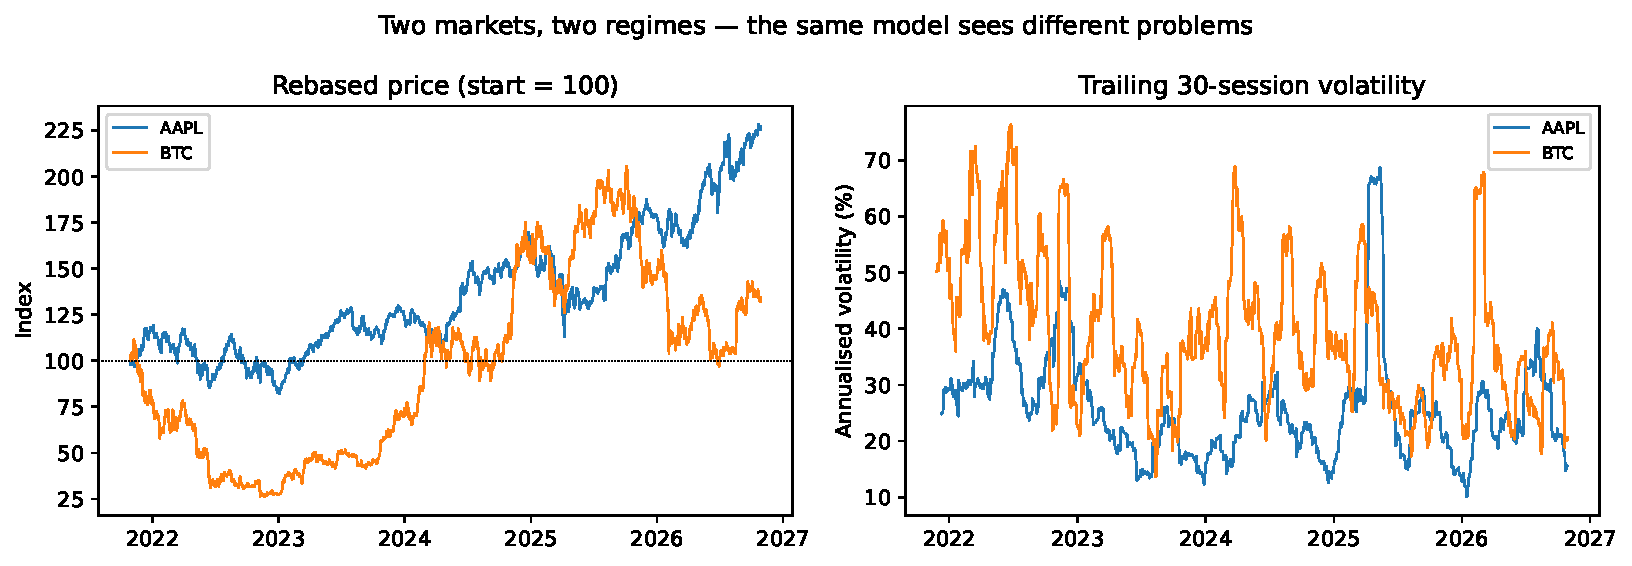
\includegraphics[width=.80\textwidth,height=.27\textheight,keepaspectratio]{fig02_asset_characteristics.pdf}
  \par
  \raggedright\scriptsize
  Full five-year history. Scales differ by over 100 times: assets are compared only with unit-free scores.
\end{frame}

% 5 ---------------------------------------------------------------------------
\begin{frame}{Selection Conditions: From Raw Bars to Modelling Rows}
  \speaker{Dong Yuankun}
  \begin{columns}[T,onlytextwidth]
    \begin{column}{.47\textwidth}
      \small\textbf{Conditions every row must meet}
      \begin{enumerate}\scriptsize\setlength{\itemsep}{2pt}
        \item \textbf{Window:} five years from 2021-10-28, after Apple's 2020 split, so raw
          prices have no split jumps.
        \item \textbf{Price field:} raw close; adjusted prices are revised later.
        \item \textbf{Quality gate:} no duplicate dates, missing values, non-positive prices,
          high below low, close outside [low, high] or negative volume. Any failure stops the
          pipeline: reject, never repair.
        \item \textbf{Complete history:} drop the first \Warmup{} rows (windows not yet full) and
          the last row (no next close).
      \end{enumerate}
    \end{column}
    \begin{column}{.49\textwidth}
      \centering\footnotesize
      \renewcommand{\arraystretch}{1.2}
      \begin{tabular}{@{}lrr@{}}
        \toprule
        & \textbf{AAPL} & \textbf{BTC} \\
        \midrule
        Raw daily bars & \ObsAAPL & \ObsBTC \\
        Quality gate & \QualityAAPL & \QualityBTC \\
        Warm-up rows & $-$\Warmup & $-$\Warmup \\
        Last row & $-1$ & $-1$ \\
        \midrule
        \textbf{Modelling rows} & \textbf{\RowsAAPL} & \textbf{\RowsBTC} \\
        \quad Train (60\%) & \TrainRowsAAPL & \TrainRowsBTC \\
        \quad Validation (20\%) & \ValidationRowsAAPL & \ValidationRowsBTC \\
        \quad Test (20\%, sealed) & \TestRowsAAPL & \TestRowsBTC \\
        \bottomrule
      \end{tabular}
      \par\vspace{1mm}
      {\scriptsize PASS: no row flagged. One row is also\\ purged at each split boundary.\par}
    \end{column}
  \end{columns}
\end{frame}

% ===================================================================== PART 2
\act{Part 2: Processing and Feature Engineering}
\progresssection{2}

% 6 ---------------------------------------------------------------------------
\begin{frame}{Problems in the Raw Data, and How We Handled Each}
  \speaker{Zhang Yancheng}
  \centering\footnotesize
  \renewcommand{\arraystretch}{1.22}
  \begin{tabular}{@{}>{\raggedright\arraybackslash}p{.27\linewidth}>{\raggedright\arraybackslash}p{.31\linewidth}>{\raggedright\arraybackslash}p{.355\linewidth}@{}}
    \toprule
    \textbf{Problem} & \textbf{Why it matters} & \textbf{What we did} \\
    \midrule
    Price levels drift and differ by asset & A model fitted on old levels cannot extrapolate to new ones & Turn prices into returns and ratios (scale-free) \\
    Adjusted prices are revised later & They carry information from the future & Use the raw close as the target \\
    Two calendars (weekends vs 24/7) & ``Next day'' means different things & Next bar on each asset's own calendar; never align rows \\
    Rolling windows need history & Partial windows or back-filling distort or leak & Drop the first \Warmup{} rows \\
    Features on different scales & Distances and penalties favour large-scale inputs & P2: standardise, fitted on training rows only \\
    Time order & A shuffled split trains on the future & Chronological split, one row purged per boundary \\
    \bottomrule
  \end{tabular}
\end{frame}

% 7 ---------------------------------------------------------------------------
\begin{frame}{From One Day's Prices to Ten Features}
  \speaker{Zhang Yancheng}
  \begin{columns}[T,onlytextwidth]
    \begin{column}{.31\textwidth}
      \footnotesize\textbf{AAPL, \ExDate{} (\FxDowName)}\par\vspace{1mm}
      \scriptsize
      \renewcommand{\arraystretch}{1.2}
      \setlength{\tabcolsep}{3pt}
      \begin{tabular}{@{}lr@{}}
        Close today & \ExCt \\
        Close yesterday & \FxPrevClose \\
        High & \FxHigh \\
        Low & \FxLow \\
        5-day average close & \FxSmaFive \\
        Volume & \FxVolM{}\,M \\
        5-day average volume & \FxVolSmaM{}\,M \\
      \end{tabular}
      \par\vspace{3mm}
      \scriptsize Only this day and earlier days are used. Next day's close is the answer, never an input.
    \end{column}
    \begin{column}{.66\textwidth}
      \centering\scriptsize
      \renewcommand{\arraystretch}{1.18}
      \setlength{\tabcolsep}{4pt}
      \begin{tabular}{@{}l>{\raggedright\arraybackslash}p{.46\linewidth}r@{}}
        \toprule
        \textbf{Feature} & \textbf{How it is computed} & \textbf{Value} \\
        \midrule
        \texttt{ret\_1} & $\ExCt / \FxPrevClose - 1$ & \FxRetOne\% \\
        \texttt{ret\_5}, \texttt{ret\_20} & Same, against 5 and 20 days ago & \FxRetFive\%, \FxRetTwenty\% \\
        \texttt{ma\_gap\_5} & $\ExCt / \FxSmaFive - 1$ & \FxGapFive\% \\
        \texttt{ma\_gap\_20} & Same, against the 20-day average & \FxGapTwenty\% \\
        \texttt{vol\_10}, \texttt{vol\_30} & Std.\ dev.\ of daily returns, last 10 and 30 days & \FxVolTen\%, \FxVolThirty\% \\
        \texttt{range\_1} & $(\FxHigh - \FxLow) / \ExCt$ & \FxRange\% \\
        \texttt{vol\_chg} & $\FxVolM / \FxVolSmaM - 1$ & \FxVolChg\% \\
        \texttt{dow} & Day of week (Monday $= 0$) & \FxDow \\
        \bottomrule
      \end{tabular}
      \par\vspace{2mm}
      \raggedright\scriptsize
      Every feature is a ratio or a spread, so none is a price level. Tested: append absurd future
      prices, rebuild, and every earlier row must stay identical.
    \end{column}
  \end{columns}
\end{frame}

% 8 ---------------------------------------------------------------------------
\begin{frame}{Every Model Gets the Same Data: One Shared Pipeline}
  \speaker{Zhang Yancheng}
  \centering
  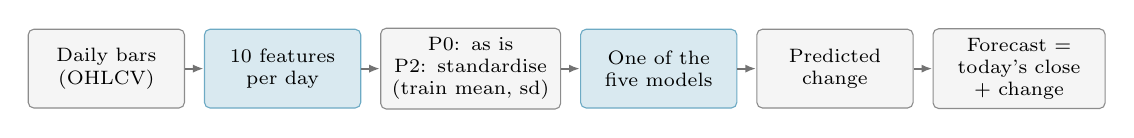
\begin{tikzpicture}[font=\scriptsize,
      box/.style={draw=black!45, fill=black!4, rounded corners=2pt, align=center,
                  minimum height=10mm, text width=1.75cm},
      key/.style={box, fill=accent!18, draw=accent!70},
      arr/.style={-{Latex[length=1.4mm]}, black!55, thick}]
    \node[box] (raw) {Daily bars\\(OHLCV)};
    \node[key, right=2.4mm of raw] (x) {\NFeatures{} features\\per day};
    \node[box, right=2.4mm of x, text width=2.05cm] (pre) {P0: as is\\P2: standardise\\(train mean, sd)};
    \node[key, right=2.4mm of pre] (m) {One of the\\five models};
    \node[box, right=2.4mm of m] (d) {Predicted\\change};
    \node[box, right=2.4mm of d, text width=1.95cm] (f) {Forecast $=$\\today's close $+$ change};
    \foreach \a/\b in {raw/x,x/pre,pre/m,m/d,d/f} \draw[arr] (\a) -- (\b);
  \end{tikzpicture}
  \par\vspace{3mm}
  \begin{columns}[T,onlytextwidth]
    \begin{column}{.52\textwidth}
      \small\textbf{Why P2 exists: very different scales}\par\vspace{1mm}
      \centering\scriptsize
      \renewcommand{\arraystretch}{1.15}
      \begin{tabular}{@{}lccc@{}}
        \toprule
        & Train sd & Raw value & After P2 \\
        \midrule
        \texttt{ret\_1} & \SdRetOne & \RawRetOne & \ZRetOne \\
        \texttt{vol\_chg} & \SdVolChg & \RawVolChg & \ZVolChg \\
        \texttt{dow} & \SdDow & \FxDow & \ZDow \\
        \bottomrule
      \end{tabular}
      \par\vspace{1mm}\raggedright\scriptsize
      Raw, \texttt{dow} is about 100 times larger than \texttt{ret\_1}: it dominates distances (SVR) and
      penalties (ridge). Trees split one feature at a time, so they do not care.
    \end{column}
    \begin{column}{.44\textwidth}
      \small\textbf{Identical for all five models}
      \begin{itemize}\scriptsize\setlength{\itemsep}{0pt}
        \item The same rows and the same \NFeatures{} columns
        \item The same target: tomorrow's close minus today's
        \item The same splits and tuning folds
        \item The same P0 or P2 setting in each run
      \end{itemize}
      \vspace{1mm}
      \scriptsize Only the learning algorithm changes. Example (\ExDate): close \ExCt, predicted change
      \ExDelta, forecast \ExPred; the next close was \ExActual.
    \end{column}
  \end{columns}
\end{frame}

% 9 ---------------------------------------------------------------------------
\begin{frame}{Chronological Split, and Proof That the Pipeline Cannot Peek}
  \speaker{Zhang Yancheng}
  \centering
  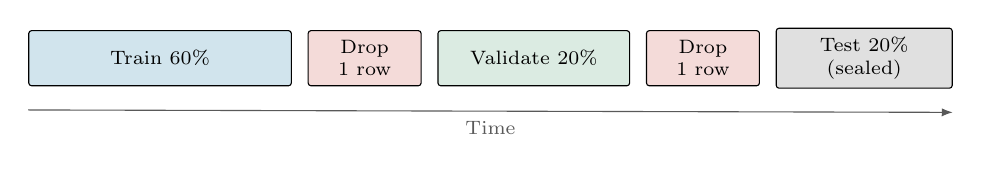
\begin{tikzpicture}[font=\scriptsize,
      seg/.style={draw, rounded corners=1pt, minimum height=7mm, align=center}]
    \node[seg, fill=accent!22, text width=3.1cm] (tr) {Train 60\%};
    \node[seg, fill=warn!18, text width=1.2cm, right=2mm of tr] (g1) {Drop 1 row};
    \node[seg, fill=good!16, text width=2.2cm, right=2mm of g1] (va) {Validate 20\%};
    \node[seg, fill=warn!18, text width=1.2cm, right=2mm of va] (g2) {Drop 1 row};
    \node[seg, fill=black!12, text width=2.0cm, right=2mm of g2] (te) {Test 20\% (sealed)};
    \draw[-{Latex[length=1.4mm]},black!65] ([yshift=-3mm]tr.south west) -- node[below]{Time} ([yshift=-3mm]te.south east);
  \end{tikzpicture}
  \par\vspace{2mm}
  \begin{columns}[T,onlytextwidth]
    \begin{column}{.50\textwidth}
      \small\textbf{Why drop a row?}\\
      \footnotesize The label is the next close, so the last training row's answer is the first
      validation price. An independent audit showed that, without the purge, changing one
      test-period price moved the headline metric by \textbf{\LeakDelta{}}.
    \end{column}
    \begin{column}{.46\textwidth}
      \small\textbf{Leakage is attacked on purpose}\\
      \footnotesize \NMutations{} known mistakes are injected one at a time (next-bar read,
      centred window, backward fill, whole-series statistic, scaler fitted on test, and a disguised
      look-ahead). \textbf{All \NMutations{} are caught}; 83 automated tests pass.
    \end{column}
  \end{columns}
  \par\vspace{2mm}
  \raggedright\footnotesize Every model-performance number in this talk comes from the validation block.
\end{frame}

% ===================================================================== PART 3
\act{Part 3: Models and Fine-Tuning}
\progresssection{3}

% 10 --------------------------------------------------------------------------
\begin{frame}{Five Models Plus a Baseline: Why Each One Is There}
  \speaker{Zhang Yancheng}
  \centering\scriptsize
  \renewcommand{\arraystretch}{1.12}
  \begin{tabular}{@{}l>{\raggedright\arraybackslash}p{.23\linewidth}>{\raggedright\arraybackslash}p{.25\linewidth}>{\raggedright\arraybackslash}p{.22\linewidth}@{}}
    \toprule
    \textbf{Model} & \textbf{How it predicts} & \textbf{Classic strength} & \textbf{Its role here} \\
    \midrule
    Naive persistence & Copies today's close & No training; hard to beat on daily prices & The yardstick \\
    Linear baseline & Weighted sum of features, small L2 penalty & Fast, transparent weights & Simplest learned model \\
    Ridge & Weighted sum, L2 penalty over a wide range & Stable with correlated inputs & Does regularisation help? \\
    SVR (RBF kernel) & Similarity to training examples & Non-linear; tolerant of small noise & Scale-sensitive case \\
    Random forest & Average of many independent trees & Non-linear, robust, little tuning & Scale-invariant control \\
    Hist.\ gradient boosting & Trees added one by one to fix remaining error & Often strongest on tabular data & Boosting vs bagging \\
    \bottomrule
  \end{tabular}
  \par\vspace{3mm}
  \raggedright\footnotesize
  Three mechanisms: linear weights, kernel similarity, tree splits. No deep learning: the course
  handout discourages it, and classical models keep the comparison interpretable.
\end{frame}

% 11 --------------------------------------------------------------------------
\begin{frame}{Fine-Tuning: The Same Search and Budget for Every Model}
  \speaker{Zhang Yancheng}
  \begin{columns}[T,onlytextwidth]
    \begin{column}{.36\textwidth}
      \centering
      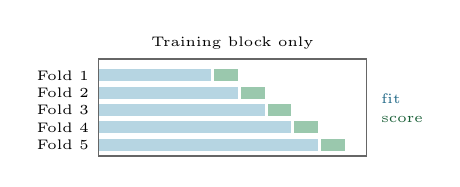
\begin{tikzpicture}[font=\tiny, x=3.4cm, y=2.2mm]
        \foreach \k/\e in {1/.52,2/.62,3/.72,4/.82,5/.92} {
          \fill[accent!35] (0,-\k) rectangle (\e-.1,-\k+.7);
          \fill[good!45] (\e-.1+.012,-\k) rectangle (\e,-\k+.7);
          \node[left] at (0,-\k+.35) {Fold \k};
        }
        \draw[black!60] (0,0.3) rectangle (1,-5.3);
        \node[above] at (.5,0.3) {Training block only};
        \node[right, text=accent!80!black] at (1.02,-2) {fit};
        \node[right, text=good!70!black] at (1.02,-3.2) {score};
      \end{tikzpicture}
    \end{column}
    \begin{column}{.60\textwidth}
      \scriptsize
      \begin{itemize}\setlength{\itemsep}{0pt}
        \item 5 expanding-window folds inside the training block, 1-row gap
        \item Random search: \TrialsUsed{} trials, $\le$\SecondsUsed{} s per cell, seed 42, for every model
        \item Objective: mean MAE across folds; the validation block is never used
        \item Grids frozen in the protocol before any result (protocol cap: \TrialsMax{} trials, \SecondsMax{} s)
      \end{itemize}
    \end{column}
  \end{columns}
  \par\vspace{2mm}
  \centering\tiny
  \setlength{\tabcolsep}{4pt}
  \renewcommand{\arraystretch}{1.1}
  % GENERATED by scripts/build_slide_assets.py -- do not edit by hand.
% Search grid per model and the configuration the inner CV chose (P2 runs).
\begin{tabular}{@{}l>{\raggedright\arraybackslash}p{.38\linewidth}>{\raggedright\arraybackslash}p{.19\linewidth}>{\raggedright\arraybackslash}p{.19\linewidth}@{}}
\toprule
Model & Grid searched & Chosen, AAPL & Chosen, BTC \\
\midrule
Linear baseline & $\alpha$ \{0.1, 1, 10\} & $\alpha$ 10 & $\alpha$ 10 \\
Ridge & $\alpha$ \{0.01, 0.1, 1, 10, 100, 1000\} & $\alpha$ 1000 & $\alpha$ 1000 \\
SVR (RBF) & C \{0.1, 1, 10, 100, 1000\}; $\varepsilon$ \{0.001, 0.01, 0.1\}; $\gamma$ \{scale, 0.001, 0.01, 0.1\} & C 0.1, $\varepsilon$ 0.1, $\gamma$ 0.01 & C 10, $\varepsilon$ 0.01, $\gamma$ 0.1 \\
Random forest & trees \{100, 200\}; depth \{None, 4, 8, 16\}; leaf \{1, 5, 20\} & trees 100, depth None, leaf 20 & trees 100, depth 4, leaf 20 \\
Hist.\ gradient boosting & lr \{0.01, 0.05, 0.1\}; iter \{100, 300\}; depth \{None, 3, 5\}; leaf \{5, 20, 50\} & lr 0.01, iter 300, depth 3, leaf 20 & lr 0.01, iter 300, depth 3, leaf 20 \\
\bottomrule
\end{tabular}

\end{frame}

% 12 --------------------------------------------------------------------------
\begin{frame}{What We Explored Beyond Hyperparameters}
  \speaker{Zhang Yancheng}
  \begin{columns}[T,onlytextwidth]
    \begin{column}{.45\textwidth}
      \small
      \textbf{1. Target representation}\\
      \footnotesize Price level first, then the change; all runs use the change.

      \vspace{1.5mm}
      \small\textbf{2. Preprocessing: P0 vs P2}\\
      \footnotesize Raw vs standardised features: 5 models $\times$ 2 assets $\times$ 2 $=$
      \NRunTotal{} runs. P1 skipped: no missing values.

      \vspace{1.5mm}
      \small\textbf{3. What scaling changed}\\
      \footnotesize Trees: identical predictions, as split thresholds predict. SVR and ridge move,
      because distances and penalties depend on scale (AAPL linear baseline MAE \LinAAPLDeltaPct\%).

      \vspace{1.5mm}
      \small\textbf{4. Grid edges}\\
      \footnotesize Ridge chose $\alpha = 1000$, the grid's edge: widening grids is a next step.
    \end{column}
    \begin{column}{.52\textwidth}
      \centering
      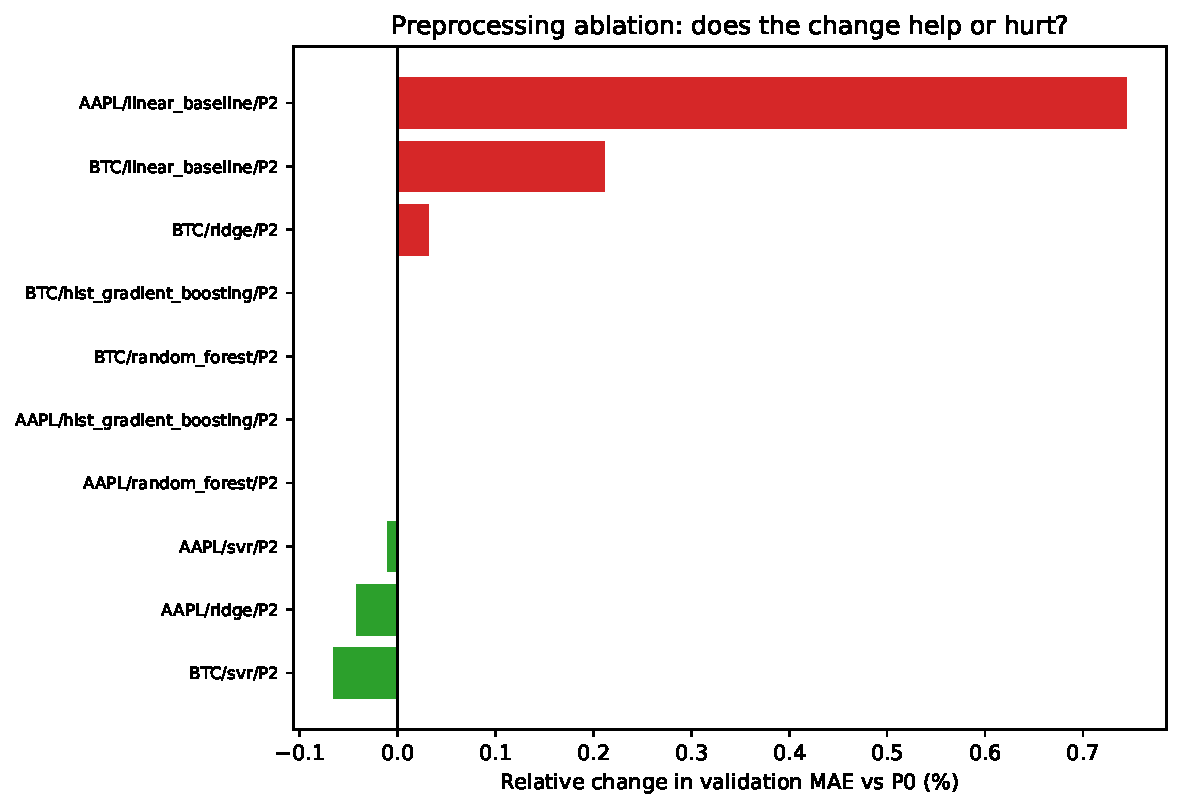
\includegraphics[width=\linewidth,height=.66\textheight,keepaspectratio]{fig06_ablation_delta.pdf}
    \end{column}
  \end{columns}
\end{frame}

% ===================================================================== PART 4
\act{Part 4: Evaluation}
\progresssection{4}

% 13 --------------------------------------------------------------------------
\begin{frame}{Four Metrics, Each With a Job}
  \speaker{Zhang Haoyu}
  \centering\footnotesize
  \renewcommand{\arraystretch}{1.18}
  \begin{tabular}{@{}l l >{\raggedright\arraybackslash}p{.30\linewidth} c c@{}}
    \toprule
    & & & \multicolumn{2}{c}{\textbf{AAPL validation}} \\
    \cmidrule(l){4-5}
    \textbf{Metric} & \textbf{Formula} & \textbf{What it tells us} & \textbf{Best (SVR)} & \textbf{Persistence} \\
    \midrule
    MAE & $\frac{1}{n}\sum |y - \hat{y}|$ & Typical error in dollars & \BestMaeAAPL & \NaiveMaeAAPL \\
    RMSE & $\sqrt{\frac{1}{n}\sum (y - \hat{y})^2}$ & Punishes large misses & \BestRmseAAPL & \NaiveRmseAAPL \\
    $R^2$ & $1 - \frac{SS_\text{res}}{SS_\text{tot}}$ & Share of price variance explained & \BestRsqAAPL & \NaiveRsqAAPL \\
    \textbf{Skill} & $1 - \frac{\text{MAE}_\text{model}}{\text{MAE}_\text{persistence}}$ & Gain over the yardstick; unit-free & \textbf{\BestAAPLSkillAll\%} & 0 \\
    \bottomrule
  \end{tabular}
  \par\vspace{2mm}
  \raggedright\footnotesize
  \begin{itemize}
    \item $R^2$ is high for any forecast that tracks yesterday's price, so it never ranks models.
    \item MAE and RMSE are in each asset's currency; only skill compares AAPL with BTC.
    \item Uncertainty: paired moving-block bootstrap intervals (slide 15).
  \end{itemize}
\end{frame}

% 14 --------------------------------------------------------------------------
\begin{frame}{Results: All \NRunTotal{} Runs Land Within 1\% of the Baseline}
  \speaker{Zhang Haoyu}
  \centering
  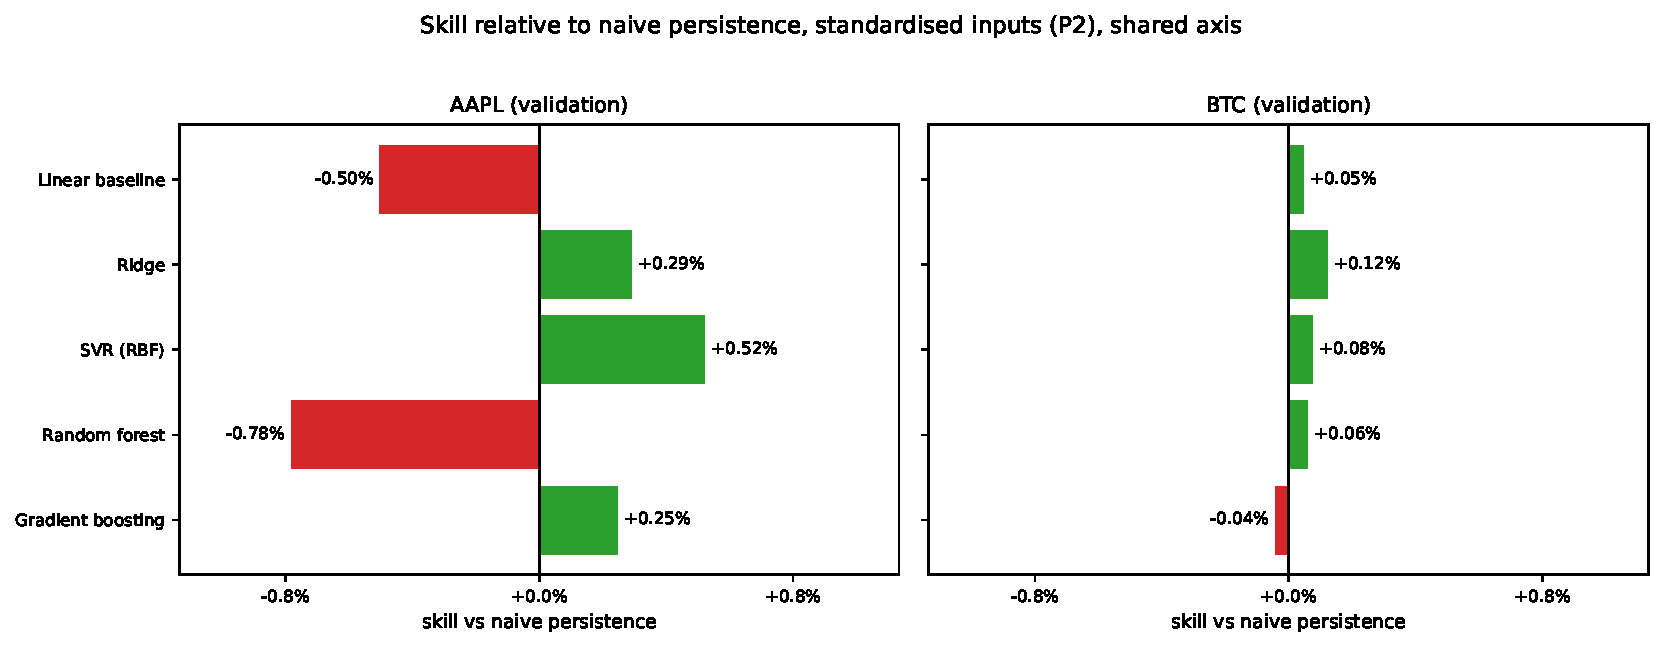
\includegraphics[width=.92\textwidth,height=.60\textheight,keepaspectratio]{fig04_model_vs_naive.pdf}
  \par\vspace{1mm}
  \raggedright\footnotesize
  \textbf{Best AAPL:} SVR (P2) \BestAAPLSkillAll\%, about \AAPLGainCents{} cents lower average error.
  \textbf{Best BTC:} linear baseline (P0) \BestBTCSkillAll\%.
  All \NRunTotal{} runs fall between \SkillMin\% and \SkillMax\% skill; \NBelowBaseline{} are below zero.
  Chart: P2 runs; the full grid is in Backup 1.
\end{frame}

% 15 --------------------------------------------------------------------------
\begin{frame}{How Certain? Every Interval Includes Zero}
  \speaker{Zhang Haoyu}
  \centering
  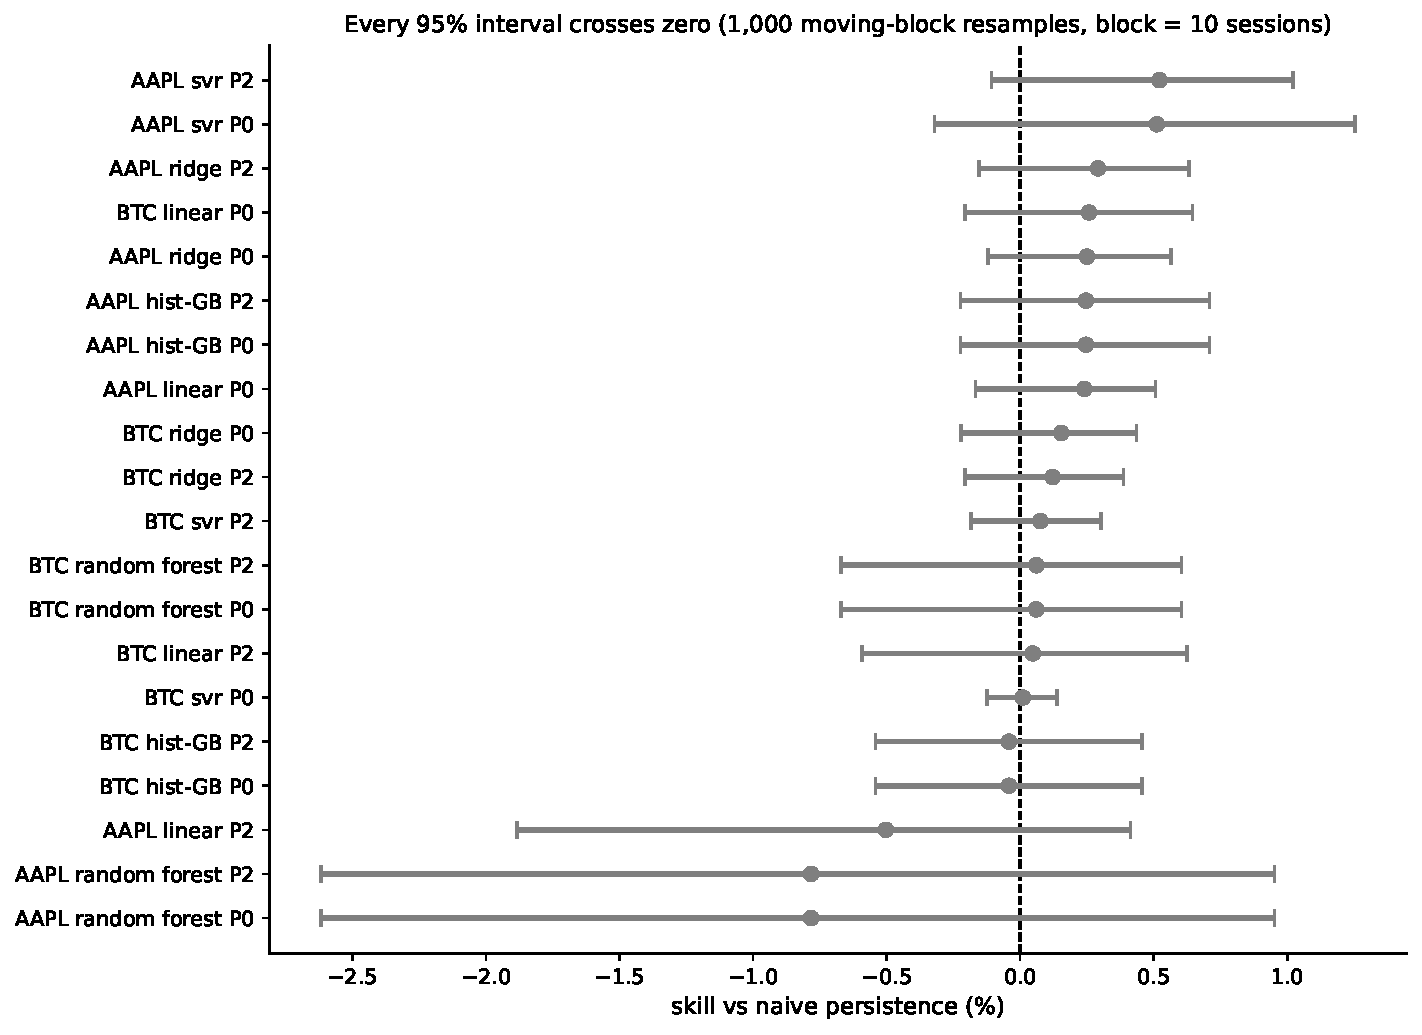
\includegraphics[width=\textwidth,height=.56\textheight,keepaspectratio]{fig08_skill_intervals.pdf}
  \par\vspace{1mm}
  \raggedright\footnotesize
  \textbf{95\% moving-block bootstrap:} errors paired by date, blocks of \CiBlock{} days,
  \CiResamples{} resamples, on \NValObsAAPL{} (AAPL) and \NValObsBTC{} (BTC) validation days.
  All \NCiIncludeZero{} intervals contain zero: parity with a strong baseline.
  \textbf{Why so hard to beat?} Consecutive daily returns are almost uncorrelated
  (AAPL \AutoAAPL, BTC \AutoBTC), so little is left to learn.
\end{frame}

% ===================================================================== PART 5
\act{Part 5: Teaching Design}
\progresssection{5}

% 16 --------------------------------------------------------------------------
\begin{frame}{Teaching Design: The Pipeline Becomes a 60-Minute Lesson}
  \speaker{Lau Pak Hei}
  \centering\scriptsize
  \renewcommand{\arraystretch}{1.25}
  \begin{tabular}{@{}l>{\raggedright\arraybackslash}p{.27\linewidth}>{\raggedright\arraybackslash}p{.22\linewidth}>{\raggedright\arraybackslash}p{.24\linewidth}@{}}
    \toprule
    \textbf{Task} & \textbf{Learners\ldots} & \textbf{From our stage} & \textbf{Course concept} \\
    \midrule
    1 & Compare training error with unseen-data error & Split (Part 2) & Fitting vs generalisation \\
    2 & Find the leak in a feature snippet & Features (Part 2) & Leakage prevention \\
    3 & Read a skill table, explain a negative value & Evaluation (Part 4) & Metrics and baselines \\
    4 & Predict which models care about scaling & Ablation (Part 3) & Train-only preprocessing, model complexity \\
    5 & Explain why low error is not profit & Limits (Part 4) & Teacher judgement \\
    \bottomrule
  \end{tabular}
  \par\vspace{3mm}
  \begin{columns}[T,onlytextwidth]
    \begin{column}{.48\textwidth}
      \footnotesize
      \textbf{Audience:} senior secondary and first-year university students new to ML.\\
      \textbf{Sequence:} hook, baseline first, then models, then discussion.
    \end{column}
    \begin{column}{.48\textwidth}
      \footnotesize
      \textbf{Materials:} Colab workbook, teacher guide with worked answers, and a notebook that
      rebuilds our results from the hashed data.
    \end{column}
  \end{columns}
\end{frame}

% 17 --------------------------------------------------------------------------
\begin{frame}{Summary: What Each Stage Delivered}
  \speaker{Lui Shing Lam}
  \centering\footnotesize
  \renewcommand{\arraystretch}{1.3}
  \begin{tabular}{@{}l>{\raggedright\arraybackslash}p{.70\linewidth}@{}}
    \toprule
    \textbf{Stage} & \textbf{Outcome} \\
    \midrule
    Data selection & Two contrasting markets, traceable sources, fingerprinted files \\
    Processing & Ten trailing features and a change target; leakage tested by \NMutations{} injected defects \\
    Models and tuning & Five mechanisms with one shared search budget and frozen grids \\
    Evaluation & All \NRunTotal{} runs within 1\% of persistence; all \NCiIncludeZero{} intervals include zero \\
    Teaching design & A 60-minute lesson with five tasks and worked answers \\
    \bottomrule
  \end{tabular}
  \par\vspace{3mm}
  \raggedright\small
  \textbf{Next steps:} open the sealed test block once; pilot the lesson with a class; widen the
  search grids; run the P3 and P4 variants.
  \par\vspace{2mm}
  {\footnotesize\bfseries Educational analysis of historical data. Not investment advice.\par}
\end{frame}

% ======================================================================= BACKUP
\progresssection{0}
\speaker{}
\appendix
\section{Backup material}
\setbeamertemplate{footline}{\intfootline}

\begin{frame}{Backup 1: Full 20-Run Transparency Matrix}
  \centering
  {\scriptsize Validation skill (\%) for every model, asset and preprocessing
   variant.\par}
  \vspace{1mm}
  \begin{center}
    \scriptsize
    \setlength{\tabcolsep}{7pt}
    % GENERATED by scripts/build_slide_assets.py -- do not edit by hand.
% Backup slide: skill (\%) for every model, asset and preprocessing variant.
\begin{tabular}{@{}lrrrr@{}}
\toprule
 & \multicolumn{2}{c}{AAPL} & \multicolumn{2}{c}{BTC} \\
\cmidrule(lr){2-3}\cmidrule(l){4-5}
Model & P0 & P2 & P0 & P2 \\
\midrule
Linear baseline & +0.24 & -0.50 & +0.26 & +0.05 \\
Ridge & +0.25 & +0.29 & +0.15 & +0.12 \\
SVR (RBF) & +0.51 & +0.52 & +0.01 & +0.08 \\
Random forest & -0.78 & -0.78 & +0.06 & +0.06 \\
Hist.\ gradient boosting & +0.25 & +0.25 & -0.04 & -0.04 \\
\midrule
Naive persistence & 0.00 & 0.00 & 0.00 & 0.00 \\
\bottomrule
\end{tabular}

  \end{center}
  {\scriptsize Highest BTC estimate overall: \BestBTCOverallConfig{} at
   \BestBTCOverallSkill\% --- its bootstrap interval includes zero.}
\end{frame}

\begin{frame}{Backup 2: Experimental Fairness and Manifest Audit}
  \begin{columns}[T]
    \begin{column}{0.5\textwidth}
      \textbf{Identical for every lane}
      \begin{itemize}\scriptsize
        \item the same 10 features, in the same order
        \item the same split boundaries and evaluation dates
        \item the same metrics and the same seed
        \item the same search budget: \TrialsUsed{} random trials,
              $\le$\SecondsUsed{}s per cell
        \item tuning scored by 5 expanding-window folds (gap 1)
              inside the training block only
      \end{itemize}
      \footnotesize
      {\scriptsize The frozen protocol permits up to \TrialsMax{} trials /
       \SecondsMax{}s; we report the budget actually used. Search is random
       over a small, declared discrete grid per model.}
    \end{column}
    \begin{column}{0.5\textwidth}
      \textbf{Every run records}
      \begin{itemize}\scriptsize
        \item run ID, git commit, dataset SHA-256
        \item protocol version and config hash
        \item hyperparameters and every attempted trial
        \item metrics, artifacts and any error trace
      \end{itemize}
      \footnotesize
      {\scriptsize Failed runs are kept, not deleted. Search grids are declared
       in the frozen protocol, before any result was seen.}
    \end{column}
  \end{columns}
\end{frame}

\begin{frame}{Backup 3: Why One Row Is Dropped at Each Boundary}
  \begin{columns}[T]
    \begin{column}{0.5\textwidth}
      \begin{block}{How the leak works}
        \scriptsize
        The label is the \emph{next} close. Without a purge, if the last training
        row were a Friday, its label would be Monday's price, which is also the
        first validation row: a training answer lives inside the validation
        block. Likewise the last validation label would be a sealed-test price.
        Nothing crashes; the score quietly improves.
      \end{block}
      \begin{block}{Fix}
        \scriptsize
        One row purged at each boundary. The loader now refuses a purge
        smaller than the forecast horizon.
      \end{block}
    \end{column}
    \begin{column}{0.5\textwidth}
      \begin{block}{What the audit measured}
        \scriptsize
        Perturbing a single test-period price moved the headline validation
        metric by \textbf{\LeakDelta{}}, far beyond any model's advantage.
      \end{block}
      \begin{block}{Mutation testing}
        \scriptsize
        \NMutations{} defects are injected one at a time: one-step look-ahead,
        disguised look-ahead, centred window, backward fill, whole-series
        statistic, preprocessing fitted on train and test.
        \textbf{All \NMutations{} are detected.} The harness was built after
        an independent audit, and it is why we can trust the pipeline.
      \end{block}
    \end{column}
  \end{columns}
\end{frame}

\begin{frame}{Backup 4: What Signals Did the Models Rely On?}
  \begin{columns}[T]
    \begin{column}{0.55\textwidth}
      \centering
      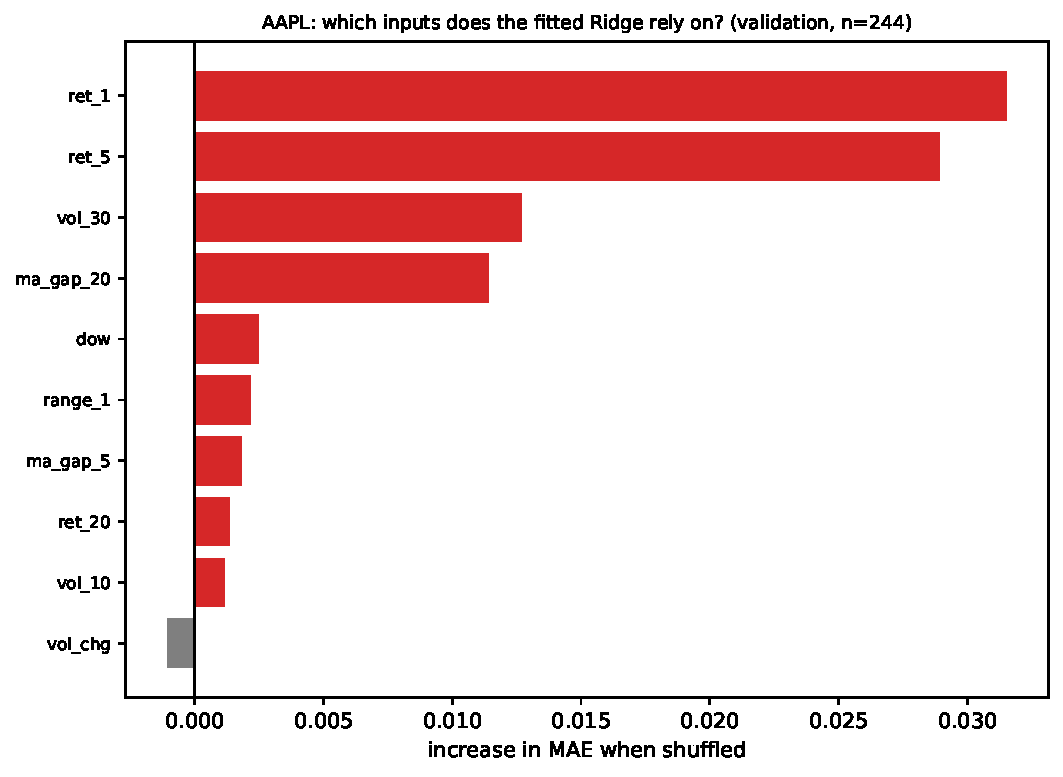
\includegraphics[width=\linewidth,height=0.66\textheight,keepaspectratio]{fig07_feature_importance_aapl.pdf}
    \end{column}
    \begin{column}{0.45\textwidth}
      \footnotesize
      Permutation importance for the ridge model on AAPL: shuffle one feature,
      measure the increase in validation error.
      \vspace{1mm}
      \begin{itemize}\footnotesize
        \item 1- and 5-day returns, 30-day volatility and the 20-day average gap matter most
        \item magnitudes are tiny --- consistent with the skill table
        \item \textbf{feature importance $\neq$ causation}
      \end{itemize}
    \end{column}
  \end{columns}
\end{frame}

\begin{frame}{Backup 5: Q\&A Quick-Reference Cards}
  \begin{table}\scriptsize
    \setlength{\tabcolsep}{4pt}
    \begin{tabular}{@{}p{0.32\textwidth}p{0.60\textwidth}@{}}
      \toprule
      Question & Answer in one line \\
      \midrule
      Why classical ML over deep learning? & The handout discourages it, and classical families keep the comparison interpretable. \\
      Does this mean markets are a pure random walk? & Lag-one return correlations are near zero, which is why a simple rule is such a strong baseline. \\
      Why compare AAPL and BTC? & One session-based equity and one 24/7 market: same protocol, different microstructure. \\
      Why P0 and P2? & They isolate the effect of scaling, the question the course cares about. P1 would duplicate P0 (no missing values); P3 and P4 are queued next. \\
      Why can the baseline have a high $R^2$? & Carrying the last close forward tracks the price level even when it misses each day's change. \\
      What does an interval including zero mean? & The model matches the baseline within measurement precision. \\
      \bottomrule
    \end{tabular}
  \end{table}
\end{frame}

\section{References}
\nocite{*}
\setbeamertemplate{bibliography item}{}
\renewcommand*{\bibfont}{\fontsize{8.5}{10.2}\selectfont}
\setlength{\bibitemsep}{2pt}

\begin{frame}{References: Models and Software}
  \printbibliography[heading=none,category=models]
\end{frame}

\begin{frame}{References: Forecasting, Evaluation and Course Materials}
  \printbibliography[heading=none,category=evaluation]
\end{frame}

\end{document}
